\subsection{Validando nosso programa}

A implementação simples do algoritmo descrito está disponível em \hyperref[https://github.com/Joao-vap/RMT-Code/blob/main/ArticleAlg/HKMC.f]{GitHub - Algoritmo Artigo}. Também fica disponível no anexo \ref{apdx: codeArtAlg}. Podemos ainda checar os ensembles clássicos e ver se podemos observar a formação da lei do semicícurlo de Wigner.

\begin{figure}
	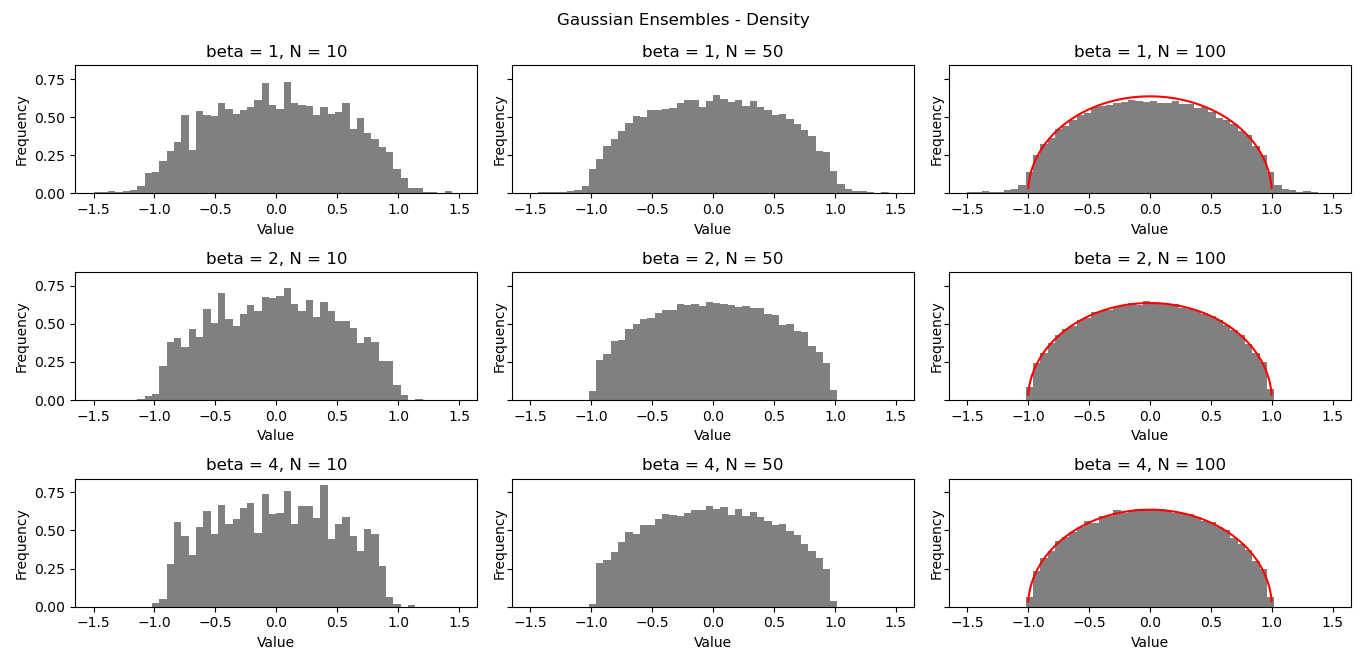
\includegraphics[scale=0.45]{images/validationArticleAlg}
	\caption{Validação para ensembles clássicos, utilizamos $200000$ passos registrando a cada $500$ a partir da metade dos passos. $\Delta t = 0.1$, $\gamma = 1$, $\alpha = 1.0$. Para replicar a semente foi $987991650$.}
\end{figure}

\subsection{Outras distribuições}

\subsubsection{Potencial Quártico}

\begin{center}
	\begin{figure}
		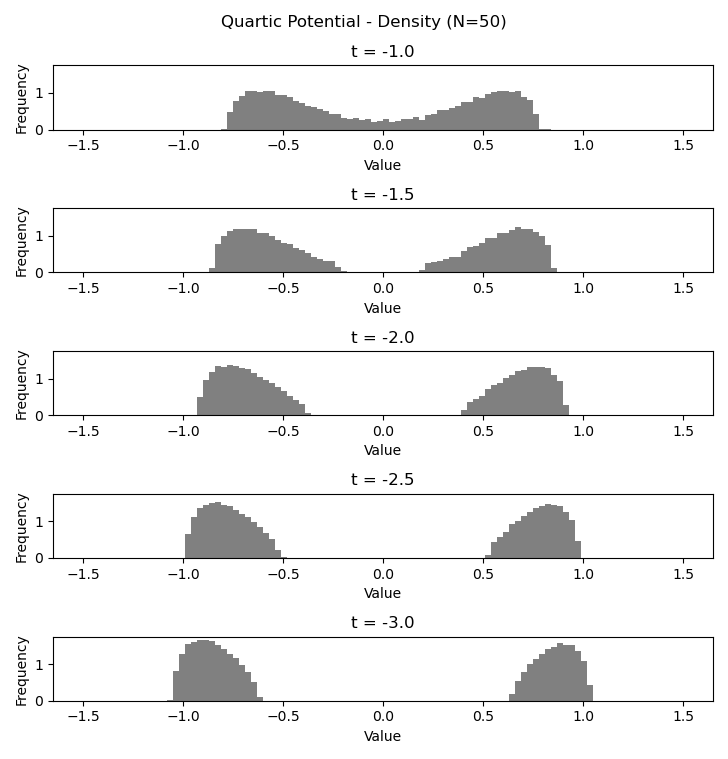
\includegraphics[scale=0.8]{images/validationArticleQuartic}
		\caption{Validação para potencial quártico, $V(x) = \frac{1}{4} x^4 + \frac{1}{2} x^2$. Utilizamos $1000000$ passos registrando a cada $500$ a partir da metade dos passos. $\Delta t = 0.1$, $\gamma = 10$, $\alpha = 0.1$. Para replicar a semente foi $987991650$.}
	\end{figure}
\end{center}

\subsubsection{Potencial Mônico}

\begin{center}
	\begin{figure}
		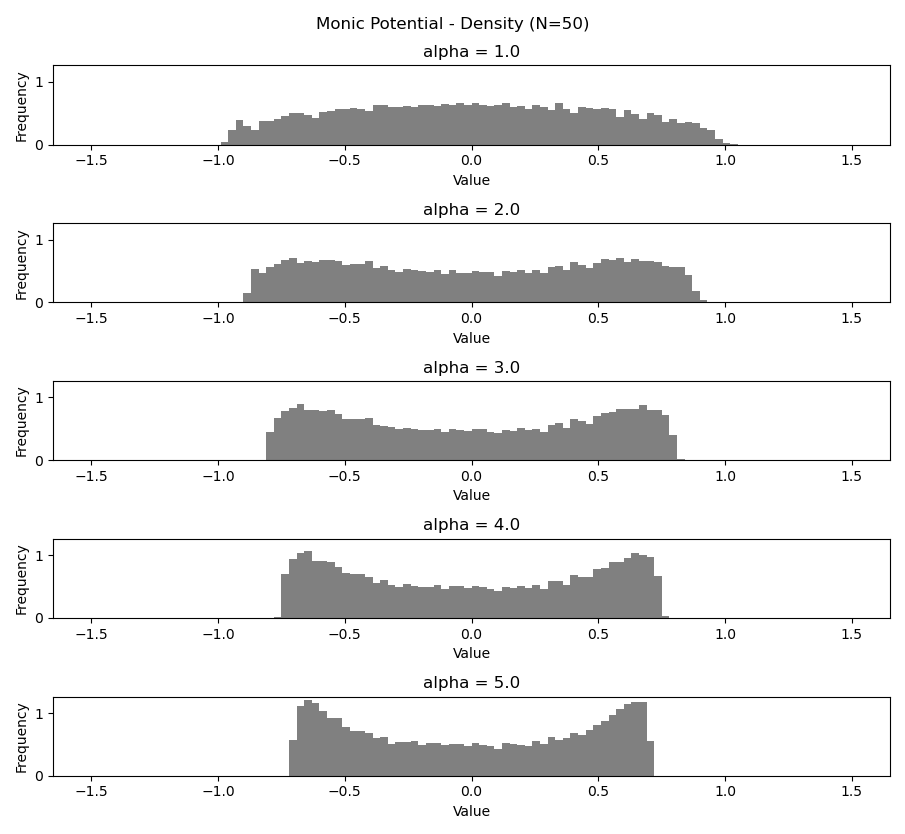
\includegraphics[scale=0.6]{images/validationArticleMonic}
		\caption{Validação para potencial mônico, $V(x) = \frac{t}{2 \alpha} x^{2\alpha}$. Utilizamos $1000000$ passos registrando a cada $500$ a partir da metade dos passos. $t = 1$, $\Delta t = 0.1$, $\gamma = 10$, $\alpha = 0.1$. Para replicar a semente foi $987991650$.}
	\end{figure}
\end{center}

\subsection{Paralelização}

